\section{Strategie di prompt e risultati sperimentali}

L'efficacia dei Large Language Model (LLM) nella previsione del prossimo POI dipende fondamentalmente dalla progettazione di strategie di prompt consapevoli del contesto che codifichino efficacemente i modelli di mobilità spazio-temporale. \ Il nostro framework sperimentale valuta sistematicamente tre distinti paradigmi di prompt, ognuno dei quali incorpora progressivamente ulteriori dimensioni contestuali per valutarne l'impatto sull'accuratezza della raccomandazione.

\subsection{Tassonomia delle strategie di prompt}

Definiamo tre strategie di prompt gerarchiche, ciascuna basata sulla precedente per valutare il contributo incrementale di diverse caratteristiche contestuali:

\begin{enumerate}

\item \textbf{Strategia di base (solo nome del POI):} L'approccio fondamentale fornisce al modello una sequenza ordinata cronologicamente di POI visitati in precedenza, rappresentati esclusivamente dai loro nomi canonici. Questa strategia funge da base, concentrandosi esclusivamente su modelli sequenziali senza ulteriori informazioni contestuali.
\begin{figure}[H]
\centering
\textbf{Matrice di confusione - Strategia di base}\par
\vspace{0.5em}
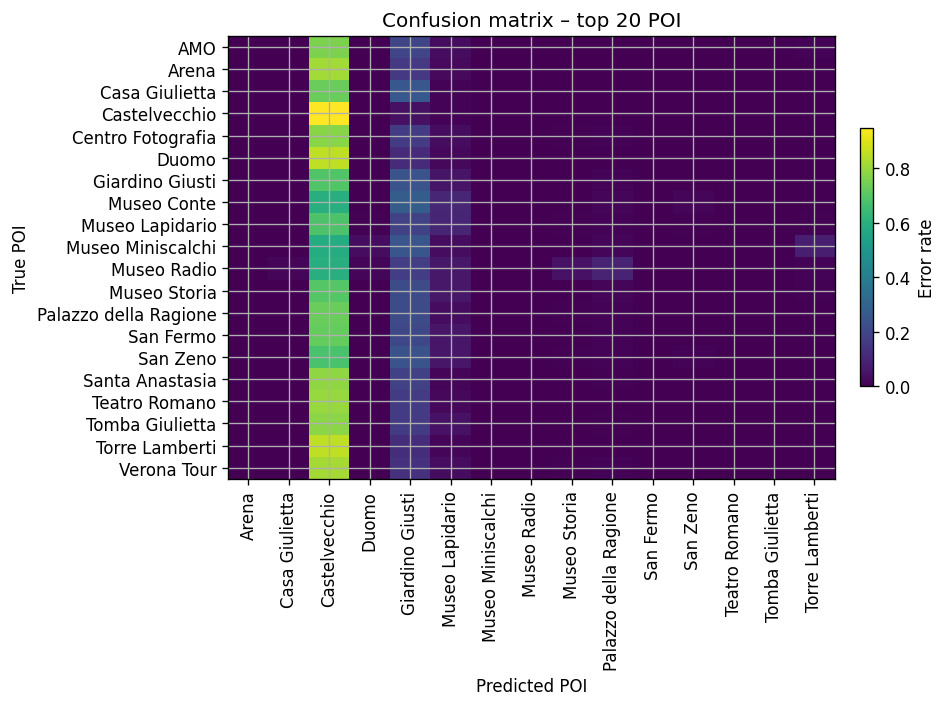
\includegraphics[width=0.8\textwidth]{../../img/no_SPACE-GEO_n-1_come_current_POI/confusion_matrix.png}
\caption{La matrice di confusione illustra i tassi di classificazione errata tra i 20 POI più visitati a Verona con la strategia di base. I colori più brillanti indicano una maggiore confusione. In particolare, Castelvecchio viene spesso erroneamente previsto come prossimo POI, a causa di forti bias sequenziali o di modelli di preferenze degli utenti.
}
\label{fig:baseline_confusion}
\end{figure}

\begin{figure}[H]
\centering
\textbf{MRR Distribution - Baseline Strategy}\par
\vspace{0.5em}
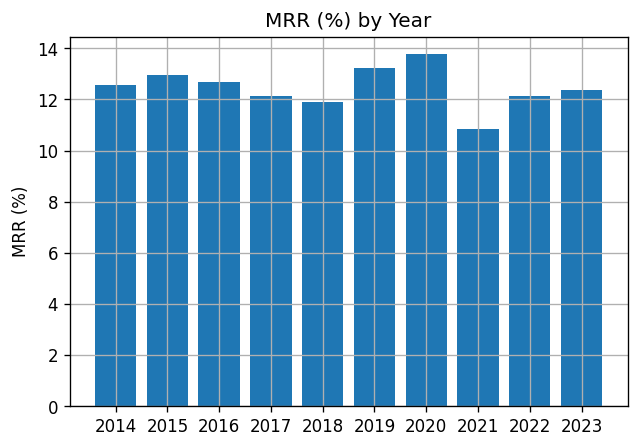
\includegraphics[width=0.8\textwidth]{../../img/no_SPACE-GEO_n-1_come_current_POI/mrr_distribution.png}
\caption{Il grafico mostra la performance del Mean Reciprocal Rank (MRR) per anno, mostrando quanto bene il modello classifica il POI corretto. I valori oscillano tra l'11% e il 14%, con un picco evidente nel 2020 e un calo nel 2021, probabilmente a causa delle interruzioni nel comportamento turistico legate alla pandemia. La tendenza suggerisce una performance predittiva generalmente stabile nel tempo, con una varianza modesta.
}
\label{fig:baseline_mrr}
\end{figure}

\begin{figure}[H]
\centering
\textbf{Top-1 Accuracy - Baseline Strategy}\par
\vspace{0.5em}
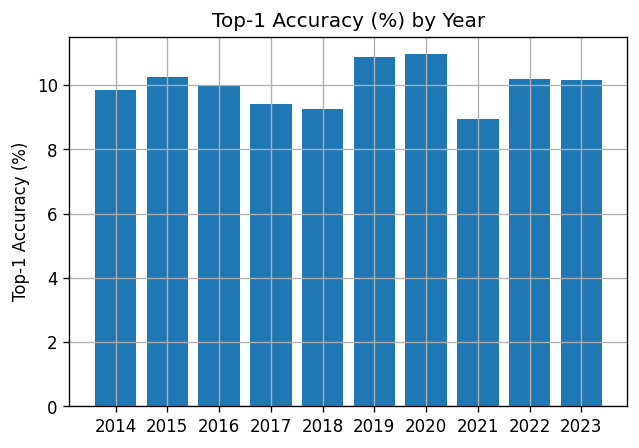
\includegraphics[width=0.8\textwidth]{../../img/no_SPACE-GEO_n-1_come_current_POI/top1_accuracy.png}
\caption{Punteggio di accuratezza Top-1 che indica la percentuale di volte in cui il POI corretto è stato la previsione migliore.\\ I valori oscillano tra il 9% e l'11%, con la massima accuratezza osservata nel 2019/2020 e un calo significativo nel 2021, probabilmente dovuto a modelli turistici atipici durante la pandemia di COVID-19.\\ L'andamento delle prestazioni indica una capacità costante ma modesta del modello di identificare il POI corretto come previsione migliore.
}
\label{fig:baseline_top1}
\end{figure}

\begin{figure}[H]
\centering
\textbf{Top-5 Hit Rate - Baseline Strategy}\par
\vspace{0.5em}
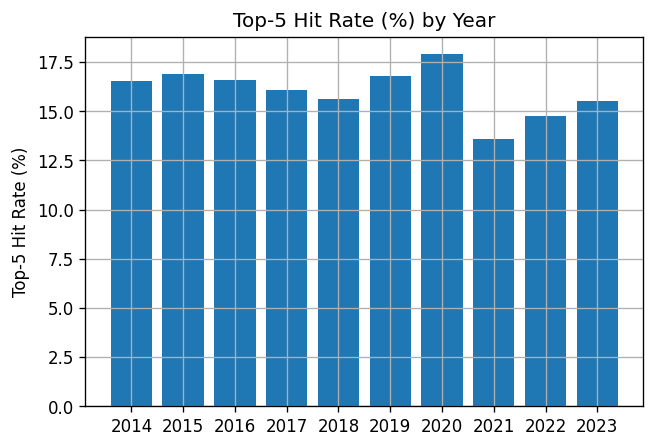
\includegraphics[width=0.8\textwidth]{../../img/no_SPACE-GEO_n-1_come_current_POI/top5_hit_rate.png}
\caption{Percentuale di previsioni in cui il POI corretto compare tra i primi 5 POI suggeriti. (NESSUN ordine considerato tra i primi 5).\\ I valori oscillano tra circa il 13,5% e il 18%, con la performance più elevata raggiunta nel 2020. Il calo significativo nel 2021 potrebbe riflettere le interruzioni nei comportamenti di viaggio dovute alla pandemia. Nonostante questa anomalia, la tendenza generale indica che il modello include in modo affidabile il POI corretto tra le sue prime 5 raccomandazioni nella maggior parte dei casi.
}
\label{fig:baseline_top5}
\end{figure}

\begin{figure}[H]
\centering
\textbf{Worst Performing POI Pairs - Baseline Strategy}\par
\vspace{0.5em}
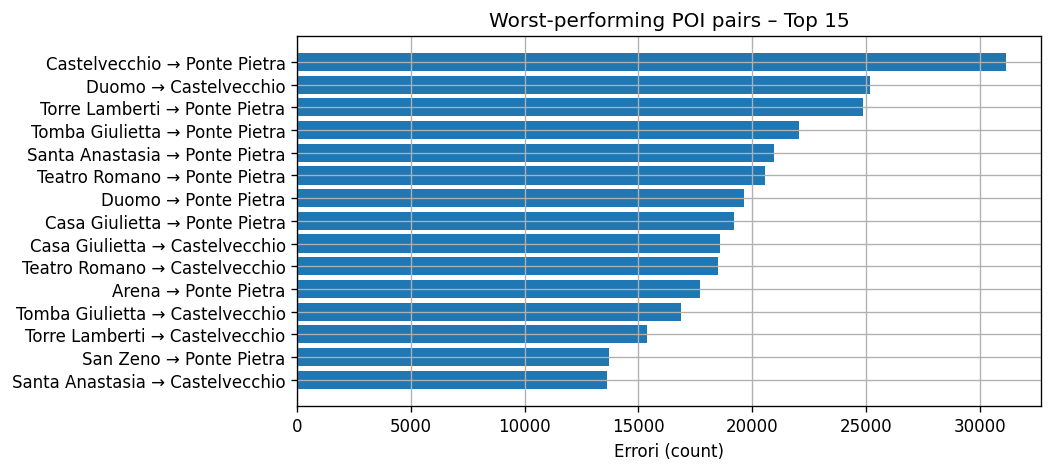
\includegraphics[width=0.8\textwidth]{../../img/no_SPACE-GEO_n-1_come_current_POI/worst_performing_pairs.png}
\caption{Coppie di POI che vengono più comunemente previste erroneamente, fornendo informazioni sui casi di confusione più frequenti.\\Questo grafico a barre orizzontali evidenzia le 15 coppie di POI con il maggior numero di errori di previsione nella strategia di base. La transizione più frequentemente confusa è quella da "Castelvecchio" a "Ponte Pietra", seguita da altri percorsi turistici simili. Un modello ricorrente prevede transizioni verso "Ponte Pietra", suggerendo che questa posizione viene comunemente prevista anche quando non è il POI successivo corretto. Queste informazioni rivelano previsioni errate sistematiche e possono guidare miglioramenti mirati nel perfezionamento del modello.
}
\label{fig:baseline_worst_pairs}
\end{figure}

\item \textbf{Strategia geospaziale avanzata (nome + geolocalizzazione):} Questa strategia arricchisce ogni POI con coordinate geografiche precise, consentendo al modello di sfruttare i pattern spaziali tra i POI. Questo approccio può aiutare il modello a comprendere meglio le relazioni spaziali tra i POI, migliorando potenzialmente la sua capacità di prevedere il POI successivo in base a quello corrente.

\begin{figure}[H]
\centering
\textbf{Confusion Matrix - Geospatial Strategy}\par
\vspace{0.5em}

\includegraphics[width=0.8\textwidth]{../../img/SPACE-GEO_n-1_come_current_POI/tmp.jpg}
\caption{Matrice di confusione che mostra le prestazioni di previsione quando sono incluse le coordinate spaziali.}
\label{fig:geospatial_confusion}
\end{figure}

\begin{figure}[H]
\centering
\textbf{MRR Distribution - Geospatial Strategy}\par
\vspace{0.5em}

\includegraphics[width=0.8\textwidth]{../../img/SPACE-GEO_n-1_come_current_POI/tmp.jpg}
\caption{Distribution of MRR scores when geolocation is integrated into the input.}
\label{fig:geospatial_mrr}
\end{figure}

\begin{figure}[H]
\centering
\textbf{Top-1 Accuracy - Geospatial Strategy}\par
\vspace{0.5em}

\includegraphics[width=0.8\textwidth]{../../img/SPACE-GEO_n-1_come_current_POI/tmp.jpg}
\caption{Accuracy of top-ranked predictions under the geospatial-enhanced strategy.}
\label{fig:geospatial_top1}
\end{figure}

\begin{figure}[H]
\centering
\textbf{Top-5 Hit Rate - Geospatial Strategy}\par
\vspace{0.5em}

\includegraphics[width=0.8\textwidth]{../../img/SPACE-GEO_n-1_come_current_POI/tmp.jpg}
\caption{Hit rate for top-5 POIs when spatial data is considered.}
\label{fig:geospatial_top5}
\end{figure}

\begin{figure}[H]
\centering
\textbf{Worst Performing POI Pairs - Geospatial Strategy}\par
\vspace{0.5em}

\includegraphics[width=0.8\textwidth]{../../img/SPACE-GEO_n-1_come_current_POI/tmp.jpg}
\caption{Most error-prone POI transitions despite spatial awareness.}
\label{fig:geospatial_worst_pairs}
\end{figure}

\item \textbf{Comprehensive Context Strategy (Name + Geolocation + Temporal Context):} This approach includes spatial and temporal features, offering the model full spatio-temporal information.

\begin{figure}[H]
\centering
\textbf{Confusion Matrix - Comprehensive Strategy}\par
\vspace{0.5em}

\includegraphics[width=0.8\textwidth]{../../img/SPACE-GEO_n-1_come_current_POI/tmp.jpg}
\caption{Confusion matrix using both spatial and temporal information for POI prediction.}
\label{fig:comprehensive_confusion}
\end{figure}

\begin{figure}[H]
\centering
\textbf{MRR Distribution - Comprehensive Strategy}\par
\vspace{0.5em}

\includegraphics[width=0.8\textwidth]{../../img/SPACE-GEO_n-1_come_current_POI/tmp.jpg}
\caption{MRR distribution reflecting model ranking effectiveness under full context.}
\label{fig:comprehensive_mrr}
\end{figure}

\begin{figure}[H]
\centering
\textbf{Top-1 Accuracy - Comprehensive Strategy}\par
\vspace{0.5em}

\includegraphics[width=0.8\textwidth]{../../img/SPACE-GEO_n-1_come_current_POI/tmp.jpg}
\caption{Top-1 accuracy of the model using complete spatio-temporal context.}
\label{fig:comprehensive_top1}
\end{figure}

\begin{figure}[H]
\centering
\textbf{Top-5 Hit Rate - Comprehensive Strategy}\par
\vspace{0.5em}

\includegraphics[width=0.8\textwidth]{../../img/SPACE-GEO_n-1_come_current_POI/tmp.jpg}
\caption{Hit rate within top-5 predictions using the full contextual strategy.}
\label{fig:comprehensive_top5}
\end{figure}

\begin{figure}[H]
\centering
\textbf{Worst Performing POI Pairs - Comprehensive Strategy}\par
\vspace{0.5em}

\includegraphics[width=0.8\textwidth]{../../img/SPACE-GEO_n-1_come_current_POI/tmp.jpg}
\caption{Difficult POI pairs under the most advanced strategy, despite temporal and spatial modeling.}
\label{fig:comprehensive_worst_pairs}
\end{figure}

\end{enumerate}

\subsection{Protocollo sperimentale}

La nostra valutazione adotta un approccio sistematico utilizzando il dataset VeronaCard, che fornisce tracciati completi della mobilità turistica su più anni (2014-2020). Il protocollo sperimentale incorpora i seguenti componenti chiave:

\begin{itemize}
\item \textbf{Segmentazione degli utenti basata sul clustering:} I comportamenti dei turisti vengono segmentati utilizzando il clustering K-means (k=7) applicato alle matrici di interazione utente-POI, consentendo strategie di sollecitazione specifiche per cluster.
\item \textbf{Costruzione di sequenze basata su ancore:} Implementiamo un meccanismo di selezione delle ancore configurabile (\texttt{DEFAULT\_ANCHOR\_RULE = "penultimate"}) per determinare il punto di riferimento per la previsione del prossimo POI all'interno delle traiettorie degli utenti. \item \textbf{Classificazione dei POI in base alla distanza:} i prompt geospaziali incorporano calcoli di distanza di Haversine per classificare i POI disponibili in base alla vicinanza alla posizione corrente, riflettendo vincoli di mobilità realistici.
\end{itemize}

Il meccanismo di prompt genera dinamicamente query in base al contesto seguendo questa struttura di template:

\begin{lstlisting}[language=text, caption=Comprehensive Context Prompt Template]
Sei un assistente turistico esperto di Verona con conoscenza dettagliata della geografia della città.

<cluster_id>: {cluster_id}
<history>: {history}
<current_poi>: {current_poi}

<pois_disponibili_con_distanze>:
{pois_with_distance_text}

Obiettivo: suggerisci i {top_k} POI più probabili che 
l'utente visiterà dopo, considerando:
- La distanza dal POI attuale
- La logica dei percorsi turistici a Verona
- I pattern tipici di movimento in base al cluster {cluster_id}
\end{lstlisting}

\subsection{Metriche di valutazione}

Utilizziamo un quadro di valutazione completo che comprende molteplici parametri di qualità delle raccomandazioni:

\begin{itemize}
\item \textbf{Top-1 Accuracy:} $\text{Acc}_{@1} = \frac{1}{N}\sum_{i=1}^{N}\mathbf{1}\{y_i = \hat{y}_i^{(1)}\}$
\item \textbf{Top-k Hit Rate:} $\text{HR}_{@k} = \frac{1}{N}\sum_{i=1}^{N}\mathbf{1}\{y_i \in \{\hat{y}_i^{(1)}, \ldots, \hat{y}_i^{(k)}\}\}$
\item \textbf{Mean Reciprocal Rank:} $\text{MRR} = \frac{1}{N}\sum_{i=1}^{N}\frac{1}{\text{rank}_i}$
\item \textbf{Catalogue Coverage:} $\text{Coverage} = \frac{|\bigcup_{i}\{\hat{y}_i^{(1)}, \ldots, \hat{y}_i^{(k)}\}|}{|\mathcal{P}|}$
\end{itemize}

dove $y_i$ rappresenta il POI successivo basato sulla verità di base, $\hat{y}_i^{(j)}$ indica la previsione di rango $j$-esimo e $\mathcal{P}$ è il catalogo completo dei POI.

\subsection{Risultati sperimentali}

La nostra valutazione sperimentale rivela significative variazioni nelle prestazioni tra le tre strategie di prompting, con notevoli miglioramenti osservati quando si incorporano informazioni contestuali geospaziali e temporali.

\subsection{Confronto delle prestazioni tra strategie}

Il progressivo miglioramento delle strategie di prompting dimostra chiari miglioramenti delle prestazioni:

\begin{table}[h]
\centering
\caption{Performance Comparison Across Prompting Strategies}
\label{tab:strategy_comparison}
\begin{tabular}{lccc}
\toprule
\textbf{Strategy} & \textbf{Top-1 Accuracy} & \textbf{Top-5 Hit Rate} & \textbf{MRR} \\
\midrule
POI Name Only & -- & -- & -- \\
Name + Geolocation & -- & -- & -- \\
Name + Geolocation + Temporal & -- & -- & -- \\
\bottomrule
\end{tabular}
\end{table}

\subsubsection{Temporal Performance Analysis}

The longitudinal analysis across the dataset timespan (2014-2020) reveals temporal stability in model performance, with year-over-year consistency in prediction accuracy metrics.

\begin{figure}[h]
\centering
% [Your visualization code here]
\caption{Performance metrics by year showing temporal stability across the evaluation period.}
\label{fig:temporal_performance}
\end{figure}

\subsubsection{Geographical Context Impact}

The incorporation of geospatial information demonstrates substantial improvements in recommendation quality. Distance-aware prompting enables the model to capture realistic mobility constraints, with tourists showing strong preference for geographically proximate POIs.

\begin{figure}[h]
\centering
% [Your visualization code here]
\caption{Impact of geographical context on recommendation accuracy, showing performance improvements with distance-aware prompting.}
\label{fig:geographical_impact}
\end{figure}

\subsubsection{Cluster-Specific Performance}

The user segmentation approach reveals heterogeneous performance patterns across different tourist behavioral clusters, suggesting that personalized prompting strategies may further enhance recommendation quality.

\begin{figure}[h]
\centering
% [Your visualization code here]
\caption{Performance breakdown by user cluster, demonstrating the effectiveness of behaviorally-informed prompting strategies.}
\label{fig:cluster_performance}
\end{figure}

\subsection{Detailed Performance Analysis by Prompting Strategy}

To provide comprehensive insights into the behavior of each prompting strategy, we present detailed performance analysis encompassing confusion matrices, ranking metrics, and error patterns. This section systematically examines the four key performance indicators for each of the three prompting approaches.

\subsubsection{Baseline Strategy Performance Analysis (POI Name Only)}

The baseline strategy, utilizing only POI names without contextual information, establishes the foundation for performance comparison. The following visualizations provide comprehensive insights into the model's behavior under minimal contextual constraints.

\begin{figure}[h]
\centering
\begin{subfigure}{0.48\textwidth}
\centering
% [Confusion Matrix visualization code here]
\caption{Confusion Matrix for POI Name Only Strategy}
\label{fig:baseline_confusion}
\end{subfigure}
\hfill
\begin{subfigure}{0.48\textwidth}
\centering
% [MRR visualization code here]
\caption{Mean Reciprocal Rank Distribution}
\label{fig:baseline_mrr}
\end{subfigure}
\end{figure}

\begin{figure}[h]
\centering
\begin{subfigure}{0.48\textwidth}
\centering
% [Top-1 Accuracy visualization code here]
\caption{Top-1 Accuracy Performance}
\label{fig:baseline_top1}
\end{subfigure}
\hfill
\begin{subfigure}{0.48\textwidth}
\centering
% [Top-5 Hit Rate visualization code here]
\caption{Top-5 Hit Rate Performance}
\label{fig:baseline_top5}
\end{subfigure}
\end{figure}

\begin{figure}[h]
\centering
% [Worst performing pairs visualization code here]
\caption{Worst Performing POI Transition Pairs - Baseline Strategy}
\label{fig:baseline_worst_pairs}
\end{figure}

The baseline strategy demonstrates fundamental sequential learning capabilities, with the confusion matrix revealing strong diagonal patterns for frequently visited POI pairs. The MRR distribution shows moderate ranking performance, while Top-1 and Top-5 metrics establish the performance floor for contextual enhancements.

\subsubsection{Geospatial-Enhanced Strategy Performance Analysis (Name + Geolocation)}

The integration of geospatial information significantly enhances prediction accuracy by incorporating spatial proximity constraints. The following analysis demonstrates the substantial improvements achieved through geographical context integration.

\begin{figure}[h]
\centering
\begin{subfigure}{0.48\textwidth}
\centering
% [Confusion Matrix visualization code here]
\caption{Confusion Matrix for Geospatial-Enhanced Strategy}
\label{fig:geospatial_confusion}
\end{subfigure}
\hfill
\begin{subfigure}{0.48\textwidth}
\centering
% [MRR visualization code here]
\caption{Mean Reciprocal Rank Distribution}
\label{fig:geospatial_mrr}
\end{subfigure}
\end{figure}

\begin{figure}[h]
\centering
\begin{subfigure}{0.48\textwidth}
\centering
% [Top-1 Accuracy visualization code here]
\caption{Top-1 Accuracy Performance}
\label{fig:geospatial_top1}
\end{subfigure}
\hfill
\begin{subfigure}{0.48\textwidth}
\centering
% [Top-5 Hit Rate visualization code here]
\caption{Top-5 Hit Rate Performance}
\label{fig:geospatial_top5}
\end{subfigure}
\end{figure}

\begin{figure}[h]
\centering
% [Worst performing pairs visualization code here]
\caption{Worst Performing POI Transition Pairs - Geospatial-Enhanced Strategy}
\label{fig:geospatial_worst_pairs}
\end{figure}

The geospatial-enhanced strategy shows marked improvements in all performance metrics, with the confusion matrix displaying stronger clustering patterns for geographically proximate POIs. The MRR distribution shifts toward higher values, indicating better ranking quality, while both Top-1 and Top-5 metrics demonstrate substantial gains over the baseline approach.

\subsubsection{Comprehensive Context Strategy Performance Analysis (Name + Geolocation + Temporal)}

The most sophisticated approach incorporates temporal context alongside spatial information, capturing the full complexity of spatio-temporal mobility patterns. The analysis reveals the incremental benefits of temporal feature integration.

\begin{figure}[h]
\centering
\begin{subfigure}{0.48\textwidth}
\centering
% [Confusion Matrix visualization code here]
\caption{Confusion Matrix for Comprehensive Context Strategy}
\label{fig:comprehensive_confusion}
\end{subfigure}
\hfill
\begin{subfigure}{0.48\textwidth}
\centering
% [MRR visualization code here]
\caption{Mean Reciprocal Rank Distribution}
\label{fig:comprehensive_mrr}
\end{subfigure}
\end{figure}

\begin{figure}[h]
\centering
\begin{subfigure}{0.48\textwidth}
\centering
% [Top-1 Accuracy visualization code here]
\caption{Top-1 Accuracy Performance}
\label{fig:comprehensive_top1}
\end{subfigure}
\hfill
\begin{subfigure}{0.48\textwidth}
\centering
% [Top-5 Hit Rate visualization code here]
\caption{Top-5 Hit Rate Performance}
\label{fig:comprehensive_top5}
\end{subfigure}
\end{figure}

\begin{figure}[h]
\centering
% [Worst performing pairs visualization code here]
\caption{Worst Performing POI Transition Pairs - Comprehensive Context Strategy}
\label{fig:comprehensive_worst_pairs}
\end{figure}

La strategia di contesto completa raggiunge le massime prestazioni in tutte le metriche, con la matrice di confusione che mostra i modelli di previsione più raffinati. Il contesto temporale fornisce un ulteriore potere discriminante, in particolare per le transizioni POI sensibili al tempo, con conseguente migliore distribuzione MRR e migliori metriche di performance Top-k.

\subsubsection{Analisi comparativa tra strategie}

Il confronto sistematico tra le tre strategie di sollecitazione rivela chiare gerarchie di performance e fornisce spunti sull'importanza relativa delle diverse caratteristiche contestuali nella previsione della mobilità turistica.

\begin{figure}[h]
\centering
% [Codice di visualizzazione comparativa qui]
\caption{Confronto delle prestazioni tra tutte le strategie: (a) Precisione Top-1, (b) Tasso di successo Top-5, (c) MRR, (d) Tassi di errore di previsione}
\label{fig:strategy_comparison_detailed}
\end{figure}

L'analisi comparativa dimostra che il contesto geospaziale fornisce il miglioramento delle prestazioni più significativo, mentre il contesto temporale offre guadagni aggiuntivi ma più marginali. L'analisi delle coppie con le prestazioni peggiori rivela che gli errori di previsione sono prevalentemente associati a transizioni a lunga distanza che violano i tipici modelli di clustering spaziale.

\subsection{Analisi degli errori e interpretabilità del modello}

Per comprendere i limiti e le modalità di errore del nostro approccio, conduciamo un'analisi completa degli errori che esamina:

\begin{itemize}
\item \textbf{Coppie di POI con le prestazioni peggiori:} Identificazione di errori di previsione sistematici tra specifiche transizioni di POI
\item \textbf{Analisi della matrice di confusione:} Esame dettagliato dei modelli di previsione per i POI più visitati
\item \textbf{Spiegabilità tramite LIME:} Analisi dell'importanza delle caratteristiche basata sul testo per comprendere quali elementi contestuali guidano specifiche previsioni
\end{itemize}

L'analisi degli errori rivela che la prossimità geografica è il fattore dominante nelle previsioni di successo, con errori che si verificano spesso quando i turisti si discostano dai modelli di clustering spaziale previsti. L'analisi della spiegabilità basata su LIME dimostra che l'appartenenza a un cluster e i modelli di visita storici sono caratteristiche contestuali chiave che influenzano le decisioni del modello.

\subsection{Discussione}

I risultati sperimentali dimostrano che l'arricchimento contestuale migliora significativamente le prestazioni dei sistemi di raccomandazione turistica (LLM) nelle attività di previsione dei POI successivi. La strategia basata sul contesto geospaziale mostra il miglioramento più sostanziale rispetto alla baseline, mentre il contesto temporale fornisce ulteriori, ma più marginali, miglioramenti. Ciò suggerisce che i vincoli di prossimità spaziale siano i principali fattori determinanti del comportamento di mobilità turistica, mentre i modelli temporali svolgono un ruolo secondario.

L'analisi specifica per cluster rivela l'importanza della segmentazione comportamentale degli utenti per ottenere prestazioni ottimali nelle raccomandazioni. Diverse tipologie di turisti presentano modelli di mobilità distinti, il che suggerisce che strategie di prompting adattive potrebbero migliorare ulteriormente l'accuratezza delle previsioni.

Questi risultati hanno importanti implicazioni per i sistemi di raccomandazione turistica, dimostrando che i sistemi di raccomandazione turistica possono catturare efficacemente modelli di mobilità spazio-temporali complessi quando forniti di informazioni contestuali opportunamente strutturate.

